\documentclass[tikz,border=3.14mm]{standalone}
\begin{document}
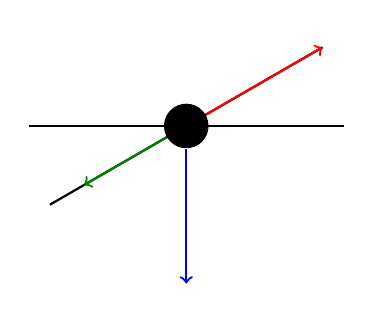
\begin{tikzpicture}

    % Define the angle of inclination 
    \def\angle{30}

    % Draw and label the slope
    \draw[thick] (-2,0) -- (2,0);
    \draw[thick, rotate=\angle] (-2,0) -- (2,0);

    % Draw and label the object (as a circle)
    \node[circle,fill,inner sep=2mm] (object) at (0,0) {};

    % Draw and label the force vectors
    \draw[blue,->,thick] (object) -- +(0,-2) node[below right] {}; % gravity (downwards)
    \draw[red,->,thick] (object) -- +(\angle:2) node[above left] {}; % normal force (perpendicular to the slope)
    \draw[green!50!black,->,thick] (object) -- +(\angle-180:1.5) node[below left] {}; % friction (upwards along slope)

\end{tikzpicture}
\end{document}